\section{Obiettivo e requisiti}

Il sistema proposto è un assistente conversazionale specializzato in
geografia, osservazione della Terra ed emergenze naturali, esposto come
\emph{Copernicus Data Workspace}. Deve interpretare richieste in linguaggio
naturale, interrogare più fonti, produrre testo e visualizzazioni e mantenere
il contesto nei turni successivi, anche riprendendo sessioni già avviate.

I requisiti che guidano l'architettura sono:

\begin{itemize}
    \item autenticare l'accesso al workspace (OIDC) e associare memoria e
    artefatti a un \texttt{thread\_id} di sessione;
    \item applicare un confine di dominio prima di effettuare chiamate esterne;
    \item selezionare una o più fonti in funzione della richiesta;
    \item distinguere Discovery sul grafo Nebula, STAC live sul catalogo remoto
    e, quando serve, il percorso combinato;
    \item eseguire in parallelo i rami operativi indipendenti;
    \item mantenere separati ragionamento, acquisizione dati e presentazione;
    \item conservare memoria e artefatti per follow-up e ripresa sessioni;
    \item presentare le acquisizioni Copernicus in una dashboard interattiva e
    modificabile senza alterare i dati di origine;
    \item continuare a fornire un risultato quando una sola sorgente fallisce;
    \item esporre un'API compatibile con OpenAI Chat Completions (SSE), usata
    dal workspace e riutilizzabile da client legacy;
    \item rendere osservabili errori, tempi e dipendenze;
    \item consentire la valutazione del workflow con riferimenti verificabili,
    controlli oggettivi e rubriche esplicite.
\end{itemize}

\section{Componenti applicativi}

L'accesso alle fonti geospaziali è mediato da un workspace conversazionale e da
un workflow persistente. I componenti vengono qui raggruppati per funzione,
mentre le dipendenze e i nodi del grafo sono descritti nelle sezioni seguenti.

\subsection{Interfaccia e API}

L'interfaccia primaria è \emph{Copernicus Data Workspace}, servita dal backend
su \path{/dashboard}. È uno spazio di lavoro a schermo intero, con home in
italiano e selettore IT/EN, in cui l'utente:

\begin{itemize}
    \item formula la domanda in linguaggio naturale (Discovery, analisi
    operativa o percorso combinato);
    \item avvia una nuova indagine oppure riprende una sessione recente che
    conserva filtri, artefatti e contesto;
    \item consulta testo, tabelle e dashboard generate dal workflow.
\end{itemize}

L'autenticazione è OIDC tramite Keycloak (realm \texttt{pecilli}). Il client
pubblico usato dal browser è \texttt{dashboard-client}. I ruoli distinguono
almeno un profilo amministratore, con accesso anche agli strumenti di
valutazione, e un profilo utente standard.

Open WebUI resta disponibile soltanto come client legacy opzionale (profilo
Compose \texttt{legacy-ui}): una Pipe può inoltrare la chat al backend nel
formato delle completion OpenAI, ma non è richiesta dal percorso standard
\cite{openWebuiDocs}. Il viewer cartografico STAC (\path{/copernicus}) resta
disponibile come vista dedicata, distinta dalla dashboard analitica.

FastAPI espone l'endpoint di chat, le API degli artefatti (lettura, mutazioni,
revisioni, chat contestuale) e lo streaming SSE. I modelli Pydantic validano
richieste, decisioni degli agenti e risultati normalizzati prima che passino al
nodo successivo \cite{fastapiDocs}. Il formato HTTP resta così separato dalla
rappresentazione interna dello stato.

\begin{figure}[htbp]
\centering
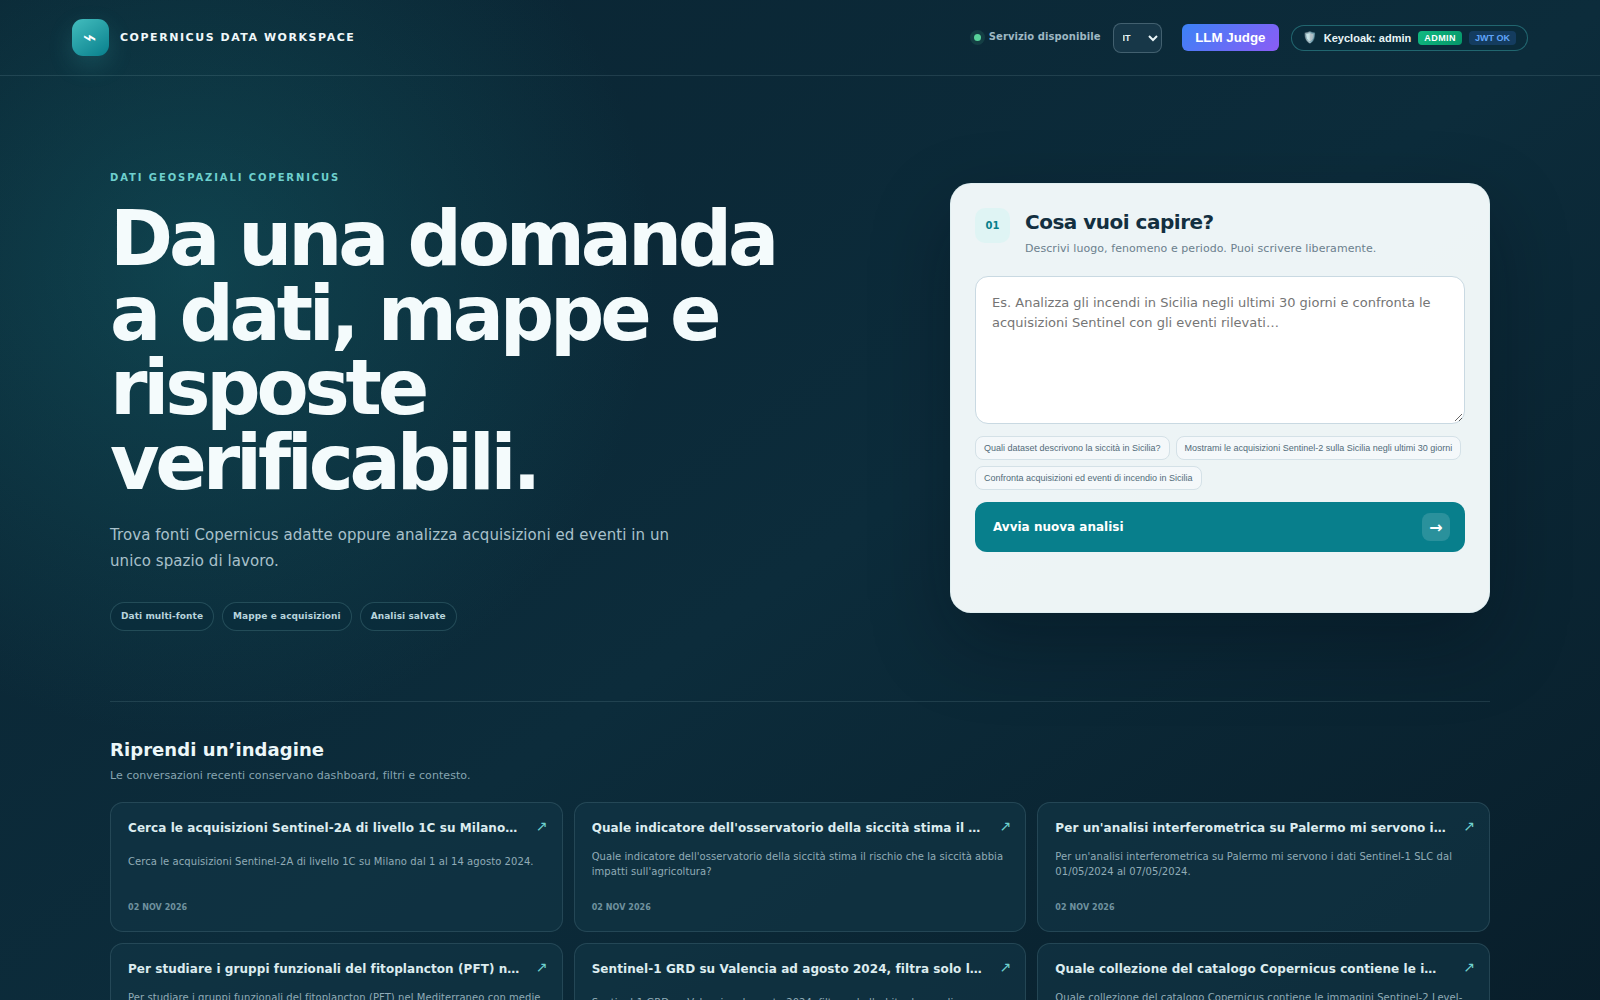
\includegraphics[width=0.92\textwidth]{Images/screenshots/ui-workspace-home.png}
\caption{Home della dashboard nativa (\emph{Copernicus Data Workspace}):
ingresso della domanda, suggerimenti, ripresa delle indagini e stato del
servizio autenticato con Keycloak.}
\label{fig:ui-workspace-home}
\end{figure}

\subsection{Orchestrazione e memoria}

LangChain gestisce messaggi, invocazioni e output strutturati del modello
\cite{langchainDocs}; LangGraph dispone le operazioni in un grafo con rami
condizionali e punti di convergenza \cite{langgraphDocs}. La scelta linguistica
determina il piano, ma è il grafo a stabilire quali nodi possano essere eseguiti
e quando i risultati siano pronti per la risposta.

Redis conserva il checkpoint associato alla conversazione: messaggi utili,
risultati raccolti, filtri e riferimenti agli artefatti. Un follow-up come
``raggruppali per giorno'' può quindi operare sul dataset precedente senza
interrogare di nuovo le sorgenti. La persistenza per thread deriva dal
checkpointer LangGraph e dalla sua integrazione Redis
\cite{langgraphPersistence,redisCheckpointer}; il riuso selettivo dei risultati
è una scelta del workflow applicativo \cite{guidaProgetto2026}. Nel percorso ordinario la
chiave deriva dal \texttt{thread\_id} della sessione workspace (e, nel client
legacy, dagli identificativi utente/chat di Open WebUI). Il fallback basato
sul primo messaggio, previsto per client privi di metadati, non offre un
isolamento adeguato a un'installazione multiutente.

\subsection{Modello e distribuzione}

Il modello servito da Ollama è remoto rispetto al backend (nel prototipo
documentato, tipicamente \texttt{qwen3:8b} per il workflow e un modello
distinto per il Judge). Riceve il contesto preparato dai nodi e interviene
nell'interpretazione, nel piano e nella risposta; non accede direttamente a
GDACS, Copernicus o Redis e non calcola i valori dei grafici. Le chiamate sono
gestite dal client applicativo mediante timeout, retry selettivi e limiti di
concorrenza, secondo la configurazione del progetto \cite{guidaProgetto2026}.
Ollama fornisce il servizio di inferenza \cite{ollamaDocs}.

Docker Compose, nella root del repository umbrella, coordina backend, asset
frontend, Keycloak, Redis, servizi MCP e infrastruttura NebulaGraph sulla rete
\texttt{pecillispace}. I profili \texttt{legacy-ui}, \texttt{harvest} e
\texttt{tools}, insieme all'overlay di osservabilità, aggiungono le rispettive
funzioni \cite{dockerComposeDocs,guidaProgetto2026}. La
Tabella~\ref{tab:tecnologie-abilitanti} riporta la responsabilità assegnata a
ciascun elemento dello stack.

\begin{table}[htbp]
\centering
\small
\begin{tabularx}{\textwidth}{
    >{\bfseries\raggedright\arraybackslash}p{0.27\textwidth}
    >{\raggedright\arraybackslash}X}
\toprule
Tecnologia & \bfseries Ruolo nel sistema \\
\midrule
Copernicus Data Workspace & Home, chat, artefatti Discovery/operativi e ripresa sessioni. \\
Keycloak & Autenticazione OIDC, realm \texttt{pecilli} e ruoli applicativi. \\
LangChain & Comunicazione strutturata tra agenti e modello linguistico. \\
LangGraph & Coordinamento dei passaggi, delle fonti e dei follow-up. \\
Redis Stack & Checkpoint per conversazione e riuso dei risultati. \\
NebulaGraph & Catalogo condiviso di metadati Marine, STAC e Drought. \\
Ollama & Inferenza del modello usato dal workflow (e, se configurato, dal Judge). \\
FastAPI e Pydantic & API del sistema e controllo della forma dei dati scambiati. \\
Docker Compose & Avvio coordinato dei servizi sulla rete \texttt{pecillispace}. \\
Prometheus e Grafana & Raccolta delle metriche e diagnosi aggregata LLMOps. \\
OpenTelemetry e Phoenix & Tracciamento delle singole esecuzioni. \\
Open WebUI (opzionale) & Client legacy di chat; profilo Compose \texttt{legacy-ui}. \\
\bottomrule
\end{tabularx}
\caption{Tecnologie del nucleo applicativo, del catalogo e dell'osservabilità.}
\label{tab:tecnologie-abilitanti}
\end{table}

\begin{figure}[htbp]
\centering
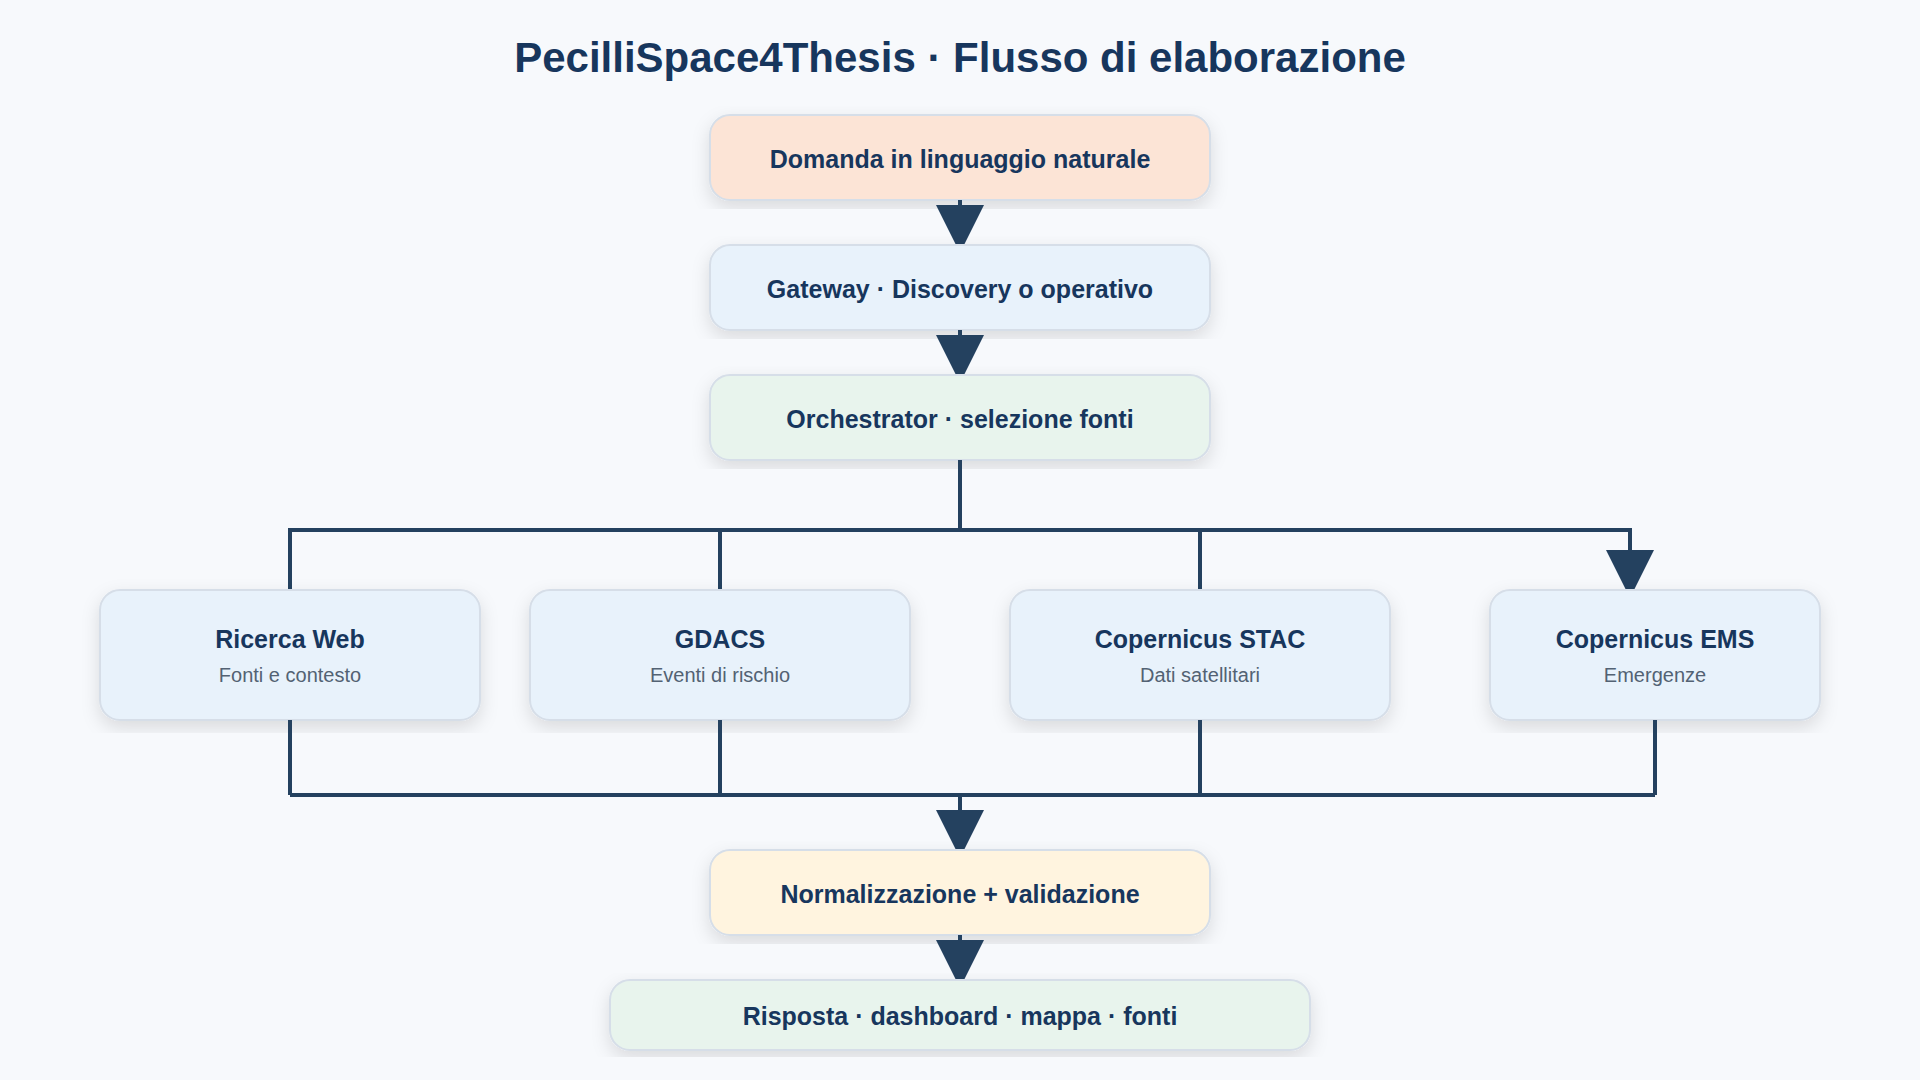
\includegraphics[width=0.88\textwidth]{Images/screenshots/diagramma_flusso.png}
\caption{Flusso di elaborazione sintetico: dalla domanda in linguaggio naturale
alla risposta con dashboard, mappa e fonti. Il gateway distingue Discovery e
percorso operativo prima della selezione delle sorgenti.}
\label{fig:diagramma-flusso}
\end{figure}

\section{Vista architetturale}

L'applicazione segue una struttura a componenti. La dashboard nativa gestisce
l'interazione con l'utente (chat, ripresa sessioni, artefatti Discovery e
acquisizioni) dopo l'accesso OIDC via Keycloak; FastAPI espone gli endpoint
della chat e degli artefatti; LangGraph coordina gli agenti; i servizi MCP e i
client dedicati accedono alle fonti esterne. La dashboard analitica delle
acquisizioni non è un testo generato dal modello: è un artefatto HTML che il
browser carica tramite API e rende a partire da un contratto JSON validato.

Il catalogo NebulaGraph aggiunge una base di metadati condivisa fra le
conversazioni, distinta dai checkpoint Redis. Gli harvester aggiornano il
catalogo; il backend lo consulta attraverso repository controllati. Metriche e
trace osservano l'esecuzione, mentre il runner del benchmark invoca lo stesso
workflow per valutarlo \cite{guidaProgetto2026}.

\begin{figure}[htbp]
\centering
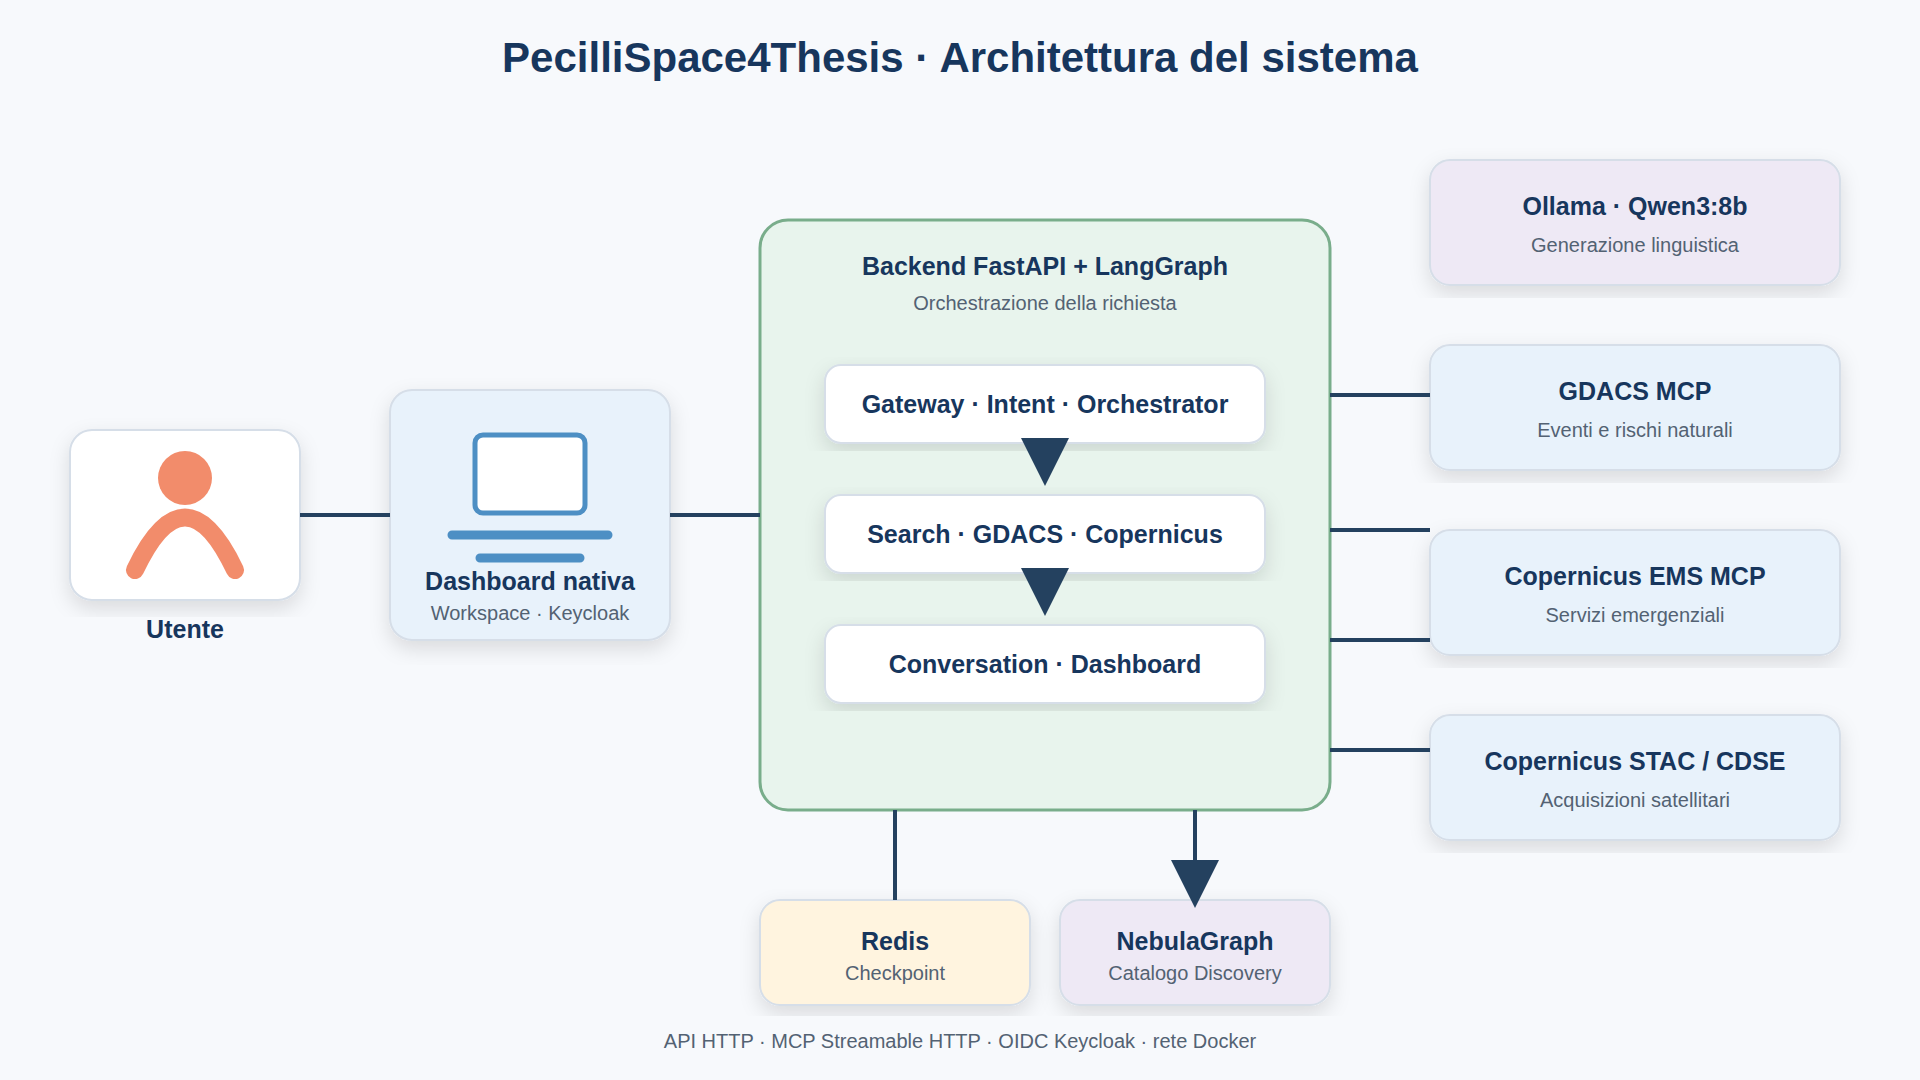
\includegraphics[width=0.95\textwidth]{Images/screenshots/architettura_microservizi.png}
\caption{Vista a componenti del prototipo: dashboard nativa autenticata,
backend LangGraph, Redis, NebulaGraph e sorgenti MCP/STAC sulla rete Docker
condivisa.}
\label{fig:architettura-microservizi}
\end{figure}

\begin{figure}[htbp]
\centering
\resizebox{0.98\textwidth}{!}{%
\begin{tikzpicture}[
    box/.style={rectangle,rounded corners,draw=blue!65!black,thick,
        fill=blue!8,align=center,minimum height=11mm,text width=31mm},
    store/.style={box,fill=violet!10,draw=violet!65!black},
    source/.style={box,fill=green!10,draw=green!45!black},
    line/.style={-{Latex[length=2mm]},thick},
    obs/.style={line,dashed,draw=orange!75!black}
]
    \node[box] (ui) at (0,0) {Dashboard nativa\\e Keycloak};
    \node[box] (api) at (4.4,0) {FastAPI};
    \node[box] (wf) at (8.8,0) {Workflow\\LangGraph};
    \node[source] (remote) at (8.8,2.3) {Web, GDACS,\\CDSE STAC, CEMS};
    \node[store] (redis) at (4.4,-2.3) {Redis e artefatti\\conversazionali};
    \node[store] (nebula) at (8.8,-2.3) {NebulaGraph\\catalogo metadati};
    \node[source] (harvest) at (8.8,-4.6) {Harvester Marine,\\STAC e Drought};
    \node[box] (llm) at (4.4,2.3) {Ollama\\modelli linguistici};
    \node[box] (obs) at (0,-2.3) {Prometheus, Grafana\\e Phoenix};
    \node[box] (eval) at (0,2.3) {Runner benchmark\\e Judge};
    \draw[line] (ui) -- (api);
    \draw[line] (api) -- (wf);
    \draw[line] (wf) -- (remote);
    \draw[line] (wf) -- (nebula);
    \draw[line] (harvest) -- (nebula);
    \draw[line] (wf.south west) -- (redis.north east);
    \draw[line] (wf.north west) -- (llm.south east);
    \draw[line] (eval.south) -- (0,1.1) -| ([xshift=-8mm]wf.north);
    \draw[obs] (api.south west) -- (obs.north east);
\end{tikzpicture}}
\caption{Componenti applicativi, catalogo e strumenti di analisi. La Discovery
legge NebulaGraph; il ramo operativo consulta le fonti remote. Il benchmark
invoca il workflow, mentre la telemetria ne osserva l'esecuzione.}
\label{fig:architettura-complessiva}
\end{figure}

Il modello linguistico non comunica direttamente con i servizi remoti. Produce
decisioni strutturate che il codice applicativo valida prima di invocare le
integrazioni e acquisirne il risultato.

I ruoli dello stack sono già riepilogati nella
Tabella~\ref{tab:tecnologie-abilitanti}. In questa architettura LangGraph e Redis
costituiscono il nucleo stateful, FastAPI espone il servizio e Pydantic delimita
i contratti. Le fonti e le dipendenze principali sono riassunte in
Figura~\ref{fig:architettura-complessiva}; ECharts e Leaflet sono invece
librerie di presentazione usate dal browser.

\section{Organizzazione del backend e del frontend}

Il backend è suddiviso secondo responsabilità esplicite:

\begin{description}
    \item[\texttt{agents/}] gateway, parsing dell'intento, orchestrazione,
    ricerca, GDACS, Copernicus STAC/CEMS, Discovery, grafici, dashboard e
    conversazione;
    \item[\texttt{api/}] route FastAPI per chat, salute, artefatti (lettura,
    mutazioni, revisioni, chat contestuale) e valutazioni;
    \item[\texttt{core/}] stato condiviso, classe base, registro, errori e
    hook di osservabilità;
    \item[\texttt{integrations/}] client CDSE/STAC, trasformazione geospaziale
    e client di lettura Nebula;
    \item[\texttt{repositories/}] query del catalogo a grafo;
    \item[\texttt{models/}] modelli Pydantic e contratti di scambio;
    \item[\texttt{services/}] MCP, risoluzione di luogo e tempo, Discovery,
    artefatti, mutazioni, health check;
    \item[\texttt{evals/}] dataset, runner, Judge e statistiche;
    \item[\texttt{workflow.py}] costruzione del grafo LangGraph.
\end{description}

Il frontend applicativo vive in \path{frontend/dashboard/} e viene servito dal
backend. I moduli principali separano chat, workspace, filtri, grafici, mappa,
tabelle, revisioni, confronti e pannello valutazioni. Il browser usa ECharts
per i grafici e Leaflet per la mappa; l'interfaccia è bilingue (IT/EN). Il
viewer STAC dedicato resta in \path{frontend/copernicus_viewer/}.

La strumentazione è raccolta nel pacchetto \texttt{copernicus\_llmops}
(\path{observability/llmops/}); gli harvester e lo schema Nebula sono sotto
\path{copernicus-harvester/}. I due server MCP sono esterni al package
applicativo e possiedono dipendenze e container autonomi: un problema del feed
GDACS non richiede di modificare il codice del ramo CEMS o STAC.

\section{Il grafo degli agenti}

\subsection{Percorso principale}

Il \texttt{WorkflowAgent} è il punto di ingresso logico. Una nuova richiesta
attraversa una parte comune e viene instradata verso Discovery o verso il
percorso operativo. Nel secondo caso il piano seleziona i worker necessari.

\begin{figure}[htbp]
\centering
\resizebox{0.93\textwidth}{!}{%
\begin{tikzpicture}[
    box/.style={rectangle,rounded corners,draw=blue!65!black,thick,
        fill=blue!8,align=center,minimum height=10mm,text width=35mm},
    line/.style={-{Latex[length=2mm]},thick}
]
    \node[box] (in) at (0,0) {Ingress e Gateway};
    \node[box] (di) at (-3,-2) {Discovery intent};
    \node[box] (oi) at (3,-2) {Intent parsing\\e piano operativo};
    \node[box] (dr) at (-3,-4) {Retrieve\\NebulaGraph};
    \node[box] (or) at (3,-4) {Worker selezionati\\Search, GDACS, STAC, CEMS};
    \node[box] (dk) at (-3,-6) {Rank deterministico\\e artefatto Discovery};
    \node[box] (oc) at (3,-6) {Raccolta e viste\\delle acquisizioni};
    \node[box] (out) at (0,-8) {Composizione e risposta};
    \draw[line] (in) -- node[above left,font=\small]{Discovery} (di);
    \draw[line] (in) -- node[above right,font=\small]{operativo} (oi);
    \draw[line] (di) -- (dr);
    \draw[line] (dr) -- (dk);
    \draw[line] (oi) -- (or);
    \draw[line] (or) -- (oc);
    \draw[line] (dk) -- (out);
    \draw[line] (oc) -- (out);
    \draw[line,dashed] (in.west) -- ++(-5.5,0) |- node[pos=0.7,below,font=\small]
        {risposta diretta fuori dominio} (out.west);
\end{tikzpicture}}
\caption{Due percorsi di una nuova richiesta ammessa. Il disegno sintetizza i
rami e omette i dettagli dei follow-up, dei nodi finali di verifica e della
dipendenza CEMS--STAC descritta nel testo.}
\label{fig:workflow-principale}
\end{figure}

Nel ramo operativo Search e Copernicus STAC costituiscono il piano di base;
GDACS e CEMS lo integrano secondo la richiesta.
LangGraph usa oggetti \texttt{Send} per creare un
\texttt{source\_worker} per ogni sorgente selezionata. Search, GDACS e STAC
possono quindi procedere contemporaneamente. Quando sono richiesti insieme
CEMS e STAC, il sistema esegue prima CEMS: l'area o le coordinate
dell'attivazione possono rendere più precisa la successiva ricerca
satellitare.

\subsection{Gateway e confine di dominio}

Il Gateway Agent classifica ogni turno, non soltanto il primo. Sono ammessi
argomenti relativi a geografia, spazio, osservazione della Terra, clima,
pericoli naturali ed emergenze. Una domanda estranea riceve una risposta diretta
e non raggiunge parser, motore di ricerca o dashboard.

Se la classificazione non è disponibile, il sistema adotta un comportamento
\emph{fail closed}: non avvia integrazioni esterne. La scelta riduce chiamate
non necessarie e impedisce che un errore del modello allarghi implicitamente il
dominio operativo.

\subsection{Parsing dell'intento}

L'Intent Parsing Agent converte il testo in una
\texttt{ResolvedRequestSchema}. Lo schema contiene:

\begin{itemize}
    \item argomenti e relativa categoria;
    \item luoghi testuali, paese, città, coordinate o bounding box;
    \item intervallo temporale normalizzato e fuso orario;
    \item obiettivo dell'analisi, filtri e aggregazioni;
    \item modalità di risposta e viste richieste.
\end{itemize}

Espressioni quali ``oggi'', ``la settimana scorsa'' o ``negli ultimi 30
giorni'' vengono trasformate in estremi temporali. Se manca un'informazione
indispensabile, il parser produce una richiesta di chiarimento; la domanda
parziale viene conservata e completata al turno successivo.

\subsection{Orchestratore e piano di esecuzione}

L'Orchestrator Agent restituisce una lista di sorgenti, non una singola classe.
Il piano ammette \texttt{search}, \texttt{gdacs}, \texttt{copernicus} e
\texttt{copernicus\_ems}. Alla decisione del modello si affiancano regole
deterministiche. Nel percorso operativo multi-sorgente qui descritto, Search e
Copernicus STAC forniscono contesto web e acquisizioni per la dashboard; questa
regola non implica l'attivazione di tali sorgenti nella Discovery. Le richieste di pericolo
aggiungono GDACS, mentre un codice CEMS esplicito aggiunge il ramo dedicato alle
attivazioni. Il workflow può inoltre applicare GDACS come fonte strutturata di
supporto quando il piano segnala un possibile pericolo.

Il risultato è una forma di orchestrazione ibrida: l'LLM gestisce la varietà
del linguaggio, mentre regole verificabili preservano i vincoli applicativi.

\subsection{Il ramo Discovery}
\label{subsec:discovery-workflow}

La Discovery usa i nodi \texttt{discovery\_intent},
\texttt{discovery\_retrieve} e \texttt{discovery\_rank}. L'agente d'intento
rappresenta tema, area, periodo, tipo di risorsa e variabili. Il servizio
\path{services/copernicus_discovery.py} espande alias di dominio, seleziona le
sorgenti e interroga \texttt{CopernicusGraphRepository}. Controlli di
compatibilità filtrano i candidati sulla base dei metadati disponibili.
Un'area incompatibile non giustifica la sostituzione silenziosa del luogo;
eventuali alternative temporali richiedono un avviso.

Il ranking è deterministico: il metodo
\texttt{CopernicusDiscoveryRankingAgent.rank()} applica la politica
\texttt{graph-score-v1}, senza sottoporre i candidati a un LLM. Lo score è
calcolato in \texttt{CopernicusDiscoveryService.\_score()} su feature
verificabili nei metadati (corrispondenza di titolo/identità/variabili,
compatibilità spaziale e temporale, tipo di risorsa, servizio preferito), con
penalità per incompatibilità e normalizzazione finale in $[0,1]$. La selezione
ammette candidati con punteggio almeno $\max(0{,}28,\mathrm{best}-0{,}20)$ e
al più 30 risorse; se sono richieste più variabili esplicite, viene forzata la
presenza di un rappresentante per ciascuna. La descrizione disponibile non riporta qui la formula completa, i pesi,
l'ordine dei candidati prima del limite e la gestione dei pareggi: soglie e
feature non bastano quindi a riprodurre lo score. Il trattamento dei metadati
assenti e la regola sulle variabili richiedono verifica nel codice prima di
interpretarli come garanzia di compatibilità. Il nome ``Agent'' identifica una
responsabilità del workflow, non un componente che effettua inferenza
linguistica.

Il repository limita ogni interrogazione a 120 righe; il servizio conserva al
massimo 30 candidati prima del ranking. Il ranking può quindi ordinare soltanto
ciò che il recupero gli consegna: qualità del retrieval e qualità
dell'ordinamento restano distinte. La ground truth del benchmark usa spesso un
target unico; una domanda di Discovery può però ammettere più risorse valide, e
il controllo critico sulla citazione deve essere interpretato rispetto
all'unicità del riferimento. In mancanza di una regola verificata sulle
alternative, un risultato valido diverso dal target può essere penalizzato:
questo è un limite del benchmark, non una prova di errore della risorsa. La risposta e l'artefatto riportano identificativi,
metadati e collegamenti delle risorse selezionate \cite{guidaProgetto2026}.

\section{Catalogo a grafo e pipeline di harvesting}
\label{sec:catalogo-grafo}

\subsection{Modello del dominio}

NebulaGraph conserva vertici, archi orientati e proprietà. I tag descrivono i
tipi dei vertici; gli edge type descrivono le relazioni. Lo space applicativo
predefinito nel Compose è \texttt{pecillispace}. La struttura logica riunisce i
tre cataloghi sotto \texttt{service:copernicus}, collegato mediante
\texttt{HAS\_SOURCE} a Marine, CDSE/STAC e Drought.

\begin{table}[htbp]
\centering
\small
\begin{tabularx}{\textwidth}{>{\bfseries\raggedright\arraybackslash}p{0.18\textwidth}
    >{\raggedright\arraybackslash}X}
\toprule
Sottografo & Entità e relazioni principali \\
\midrule
Marine & Product, Dataset, Version, Part, DataService, Variable e Coordinate;
Operation e Parameter documentano l'accesso. \\
\addlinespace
CDSE/STAC & StacCatalog, StacCollection, StacQueryable, StacItem e StacAsset;
gli asset conservano riferimenti ai file. \\
\addlinespace
Drought & OgcService, DroughtLayer, DroughtCoverage e DroughtTimeExtent;
sono rappresentate gerarchie dei layer e disponibilità temporali. \\
\bottomrule
\end{tabularx}
\caption{Articolazione del catalogo condiviso di metadati.}
\label{tab:sottografi}
\end{table}

Gli identificativi deterministici hanno prefissi di dominio per separare le
sorgenti. Un dataset Marine è collegato alle sue variabili direttamente e
attraverso il contesto di versioni e servizi di accesso. La radice comune
permette la navigazione fra cataloghi, ma non costituisce un'ontologia di
equivalenze fra ogni variabile Marine e ogni indicatore Drought.

\subsection{Raccolta, aggiornamento e riconciliazione}

Ogni harvester raccoglie e normalizza i metadati in un
\texttt{GraphPayload}, poi il repository esegue upsert di vertici e archi.
Le definizioni operative dello schema sono nei file
\path{marine/app/graph/schema.ngql}, \path{space/app/schema.ngql} e
\path{drought/app/schema.ngql}, relativi a \path{copernicus-harvester/}.
I file numerati sotto \path{nebula/schema/} dello stesso harvester sono
segnaposto nella revisione documentata: non vanno confusi con gli schemi
effettivamente applicati.

I campi \texttt{first\_seen\_at}, \texttt{last\_seen\_at} e
\texttt{last\_harvested\_at} descrivono prima osservazione, ultima presenza e
ultima elaborazione; \texttt{metadata\_hash} permette di riconoscere cambiamenti.
La riconciliazione può mantenere risorse scomparse con \texttt{active=false}.
Per una vista corrente occorre filtrare sia vertici sia archi attivi.

Sono presenti protezioni contro rimozioni anomale: la soglia predefinita è il
25\%, applicata a categorie Marine con almeno 20 vertici, collezioni STAC con
almeno 10 e layer Drought con almeno 5. Gli item STAC sono accumulati per
finestre incrementali: l'assenza in una finestra recente non ne prova la
scomparsa dal catalogo globale. Un limite di sicurezza raggiunto deve emergere
come errore, anziché essere presentato come raccolta completa.

L'aggiornamento a batch non offre un'atomicità globale dell'harvest: un guasto
può lasciare alcuni batch già salvati. Inoltre gli upsert aggiornano proprietà
correnti, senza conservare tutte le revisioni precedenti. Timestamp e flag di
attività rendono lo stato ispezionabile, ma non permettono di ricostruire
qualsiasi snapshot storico.

La pianificazione del profilo \texttt{harvest} prevede Marine alle 02:00, STAC
alle 03:00 e Drought alle 03:30, con fuso predefinito Europe/Rome. Lock,
timeout, tentativi limitati e file di stato controllano l'esecuzione; la salute
del catalogo richiede anche la freschezza dell'ultimo job riuscito, oltre alla
raggiungibilità del database \cite{guidaProgetto2026}.

\subsection{Infrastruttura e confine di lettura}

NebulaGraph separa gestione dello schema (\texttt{metad}), conservazione dei
dati (\texttt{storaged}) ed esecuzione delle query (\texttt{graphd})
\cite{nebulaArchitecture}. Il Compose usa la versione predefinita 3.8.0, un
servizio per ruolo e volumi persistenti per metadati e storage. Lo space creato
dal client Marine prevede dieci partizioni, identificativi
\texttt{FIXED\_STRING(256)} e \texttt{replica\_factor=1}: la separazione dei
processi non fornisce da sola alta disponibilità.

I container si collegano a \texttt{nebula-graphd:9669}; dall'host la porta è
pubblicata secondo \texttt{NEBULA\_HOST\_PORT}. Il servizio
\texttt{nebula-storage-activator} registra lo storage e termina con successo;
il suo stato normale è quindi un processo concluso. Occorre inoltre allineare
\texttt{NEBULA\_SPACE}: il default Marine fuori Compose è
\texttt{copernicus}, diverso da quello del backend.

La Discovery usa query predisposte dal codice, tramite
\path{repositories/copernicus_graph.py} e
\path{integrations/nebula/client.py}. \texttt{NebulaReadClient} ammette i
prefissi di lettura \texttt{MATCH}, \texttt{GO}, \texttt{FETCH} e
\texttt{SHOW}, blocca istruzioni multiple e mutazioni fuori dai letterali e
valida i parametri. Il modello non consegna al database uno script nGQL
arbitrario. Il vincolo è applicativo: l'utente predefinito del Compose è
\texttt{root}, quindi non dimostra una restrizione equivalente dei privilegi
del database.

\section{Agenti specializzati e nodi di elaborazione}

Nel codice molti componenti portano il suffisso ``Agent'', ma solo alcuni usano
un LLM per decidere. La Tabella~\ref{tab:agenti-llm} distingue nodi decisionali
linguistici da servizi e trasformazioni deterministiche, così che il titolo
multiagentico non venga letto come ``ogni nodo ragiona con un modello''.

\begin{table}[htbp]
\centering
\small
\begin{tabularx}{\textwidth}{
    >{\bfseries\raggedright\arraybackslash}p{0.22\textwidth}
    >{\centering\arraybackslash}p{0.12\textwidth}
    >{\raggedright\arraybackslash}p{0.28\textwidth}
    >{\raggedright\arraybackslash}X}
\toprule
Componente & LLM? & Decide cosa fare? & Operazione principale \\
\midrule
Gateway & Sì & Sì (dominio/route) & Classificazione della richiesta \\
\addlinespace[1pt]
Discovery intent & Sì & Sì (intento catalogo) & Estrazione tema/area/periodo \\
\addlinespace[1pt]
Intent / Orchestrator & Sì & Sì (piano fonti) & Parametri e selezione sorgenti \\
\addlinespace[1pt]
Discovery retrieve & No & No & Query Nebula parametrizzate \\
\addlinespace[1pt]
Discovery rank & No & Secondo regole fisse & Ordinamento \texttt{graph-score-v1} \\
\addlinespace[1pt]
Worker fonti & Ibrido & Esecuzione del piano & Recupero Search, GDACS, STAC e CEMS \\
\addlinespace[1pt]
Chart & Opzionale & Configurazione viste & Aggregazioni da record e rifinitura della vista \\
\addlinespace[1pt]
Validator & No & No & Controlli strutturali sulle viste \\
\addlinespace[1pt]
Conversation & Sì & Sì (sintesi/follow-up) & Composizione della risposta \\
\bottomrule
\end{tabularx}
\caption{Componenti del workflow: uso di LLM, potere decisionale e operazione.
``Ibrido'' indica un nodo che può usare il modello per parametri, ma esegue
recupero e filtri nel codice.}
\label{tab:agenti-llm}
\end{table}

In sintesi, gli agenti decisionali linguistici sono concentrati in gateway,
parsing/intento, orchestrazione e conversazione; ranking, repository, filtri
STAC e validazione delle viste sono elaborazioni deterministiche.

\section{Contratti e stato condiviso}

Gli agenti decisionali producono structured output validato da Pydantic. Questa
scelta separa due linguaggi:

\begin{itemize}
    \item JSON tipizzato per lo scambio interno;
    \item Markdown in linguaggio naturale per l'utente.
\end{itemize}

Lo stato LangGraph estende \texttt{MessagesState} e contiene richiesta
risolta, piano, azione di follow-up, risultati delle quattro fonti, grafici,
dashboard e risposta finale. Per la dashboard conserva inoltre filtri collegati,
stato visuale, revisioni e conversazioni contestuali per settore. Ogni campo è
associato a un \texttt{thread\_id}, che separa logicamente i checkpoint.
L'isolamento tra utenti richiede inoltre l'autorizzazione sull'identificativo
di conversazione e sugli artefatti; il solo nome della chiave non la dimostra.

Il ramo Discovery aggiunge intento, risorse recuperate e selezionate e
riferimento al proprio artefatto. Questi dati appartengono al contesto della
conversazione; il catalogo NebulaGraph resta invece una base persistente
condivisa, aggiornata dagli harvester.

I risultati delle sorgenti seguono un'impostazione comune: stato
dell'operazione, dataset normalizzato, aggregazioni, fonti ed eventuali
informazioni di errore. Il Conversation Agent non deve conoscere il formato
originale di RSS, STAC o CEMS.

\section{Persistenza}

La persistenza separa due bisogni: riprendere una conversazione e conservare
artefatti troppo grandi per il prompt. Nessuno dei due meccanismi sostituisce da
solo i controlli di autorizzazione dell'utente autenticato.

\subsection{Checkpoint conversazionali}

Redis Stack è l'unico backend della memoria conversazionale. Il
\texttt{AsyncRedisSaver} di LangGraph salva messaggi e stato dopo i nodi del
grafo. A ogni nuova richiesta il checkpoint del relativo
\texttt{thread\_id} viene ricaricato automaticamente. Se Redis non è
configurato o non è raggiungibile, il backend non viene dichiarato pronto.

La cronologia attiva è limitata agli ultimi messaggi utili, mentre i risultati
strutturati restano nello stato, evitando una crescita indefinita del prompt.

\subsection{Archivio degli artefatti}

Le heatmap e i payload della dashboard possono essere più grandi della memoria
testuale. Sono quindi salvati come artefatti JSON in un archivio dedicato. Lo
stato conserva l'identificativo; il browser legge l'artefatto con
\texttt{GET /api/dashboards/\{id\}} e invia mutazioni controllate a endpoint
dedicati. Ogni modifica crea una revisione che può essere confrontata,
annullata o ripristinata. In caso di indisponibilità temporanea di CDSE, il
servizio può cercare un artefatto precedente compatibile per area, collezione
e intervallo temporale, dichiarandone il riuso.

\section{Dashboard generativa e verificabile}

Nel percorso operativo il workflow produce una dashboard analitica a partire
dai soli record STAC Copernicus normalizzati; nel workspace essa compare come
artefatto del percorso ``Analisi dati Copernicus''. La Discovery presenta
invece risorse del catalogo a grafo (``Ricerca dati Copernicus''). Search,
GDACS e CEMS rimangono fonti della risposta testuale o di sezioni dedicate e
non alimentano le serie quantitative della dashboard STAC. La provenienza dei
valori resta così esplicita e non vengono confrontate nello stesso grafico
grandezze eterogenee.

L'artefatto contiene KPI, grafici a barre, linee o torta, tabella, heatmap e
provenienza: campi usati, filtri attivi, metodo di aggregazione, numero di
record e identificativi dei prodotti. L'LLM può scegliere o pianificare una
vista, ma il backend ricalcola conteggi, percentuali, medie, variazioni e
confronti sui record; non accetta valori numerici prodotti liberamente dal
modello.

I controlli consentono di cambiare tipo di grafico, ordinamento, Top~N,
visibilità e filtro. Un click su grafico o tabella può attivare un
cross-filter: backend e interfaccia ricalcolano coerentemente grafici, KPI,
tabella e heatmap. La chat contestuale di ciascun settore risponde sul
risultato corrente e può richiedere una mutazione tipizzata; usa la ricerca
web solo quando la domanda richiede contesto esterno non deducibile dai dati
visualizzati.

\subsection{Leggibilità e correttezza dei grafici}
\label{subsec:leggibilita-grafici}

La dashboard applica regole di rendering per evitare che una visualizzazione
formalmente corretta diventi illeggibile. I grafici temporali, quelli con più
di otto categorie e il grafico primario occupano l'intera riga; gli altri sono
disposti in una griglia responsiva. Per molte categorie sono disponibili
scorrimento e zoom; le etichette vengono troncate, ruotate quando necessario e
rese non sovrapposte. Le torte mostrano etichette esterne soltanto fino a sei
categorie e usano una legenda scorrevole; le barre orizzontali aumentano
dinamicamente l'altezza. Il renderer osserva inoltre i cambiamenti di dimensione
del contenitore e ridimensiona ECharts dopo il caricamento e quando la sezione
viene riaperta.

Queste regole non sostituiscono la validazione semantica: prima di salvare una
modifica, il Validator controlla l'allineamento di etichette, valori e serie.
Un valore mancante e uno zero osservato hanno significati diversi: una
riparazione di formato non deve essere interpretata come recupero del dato.
La validazione del payload è strutturale e non costituisce da sola una
garanzia di correttezza semantica dei dati.
Ogni grafico offre anche una tabella dei
dati e l'esportazione CSV, così che il risultato visivo resti verificabile.

\section{Integrazione MCP}

I server GDACS e CEMS usano FastMCP e il trasporto Streamable HTTP. Il backend
scopre e invoca i tool tramite un client comune. Gli strumenti principali sono:

\begin{itemize}
    \item elenco degli eventi GDACS recenti, filtrato per pericolo e finestra;
    \item dettaglio di un evento GDACS ufficiale;
    \item catalogo delle operazioni CEMS;
    \item elenco, sintesi e dettaglio delle attivazioni CEMS.
\end{itemize}

Gli indirizzi interni e le credenziali restano nella configurazione dei
servizi e non vengono passati al modello. I collegamenti pubblici ai prodotti
o alle schede ufficiali possono invece comparire nei risultati. Il client applica timeout; i servizi applicano retry
limitati agli errori transitori, evitando di ripetere richieste errate.

\section{Distribuzione tramite container}

La distribuzione comprende servizi applicativi e catalogo condiviso:

\begin{enumerate}
    \item dashboard nativa (asset statici serviti dal backend);
    \item Keycloak per OIDC e realm \texttt{pecilli};
    \item backend FastAPI;
    \item server MCP GDACS;
    \item server MCP CEMS;
    \item Redis Stack;
    \item NebulaGraph con metad, storaged, graphd e attivatore dello storage.
\end{enumerate}

Il modello Ollama è raggiunto come dipendenza esterna. I server MCP sono
visibili sulla rete interna; l'utente accede alla dashboard su
\url{http://localhost:8080/dashboard} e, se attivato, al client legacy Open
WebUI. Il backend dipende anche dal completamento dell'attivatore; le
dipendenze usano condizioni di avvio e, per i servizi predisposti, health check. Il profilo
\texttt{harvest} abilita job e schedulatori, mentre l'overlay
\path{observability/docker-compose.observability.yml} aggiunge Prometheus,
Grafana e Phoenix e avvia il backend con strumentazione. Liveness e readiness
sono separate; un processo vivo ma privo di memoria non viene considerato pronto.

\begin{figure}[htbp]
\centering
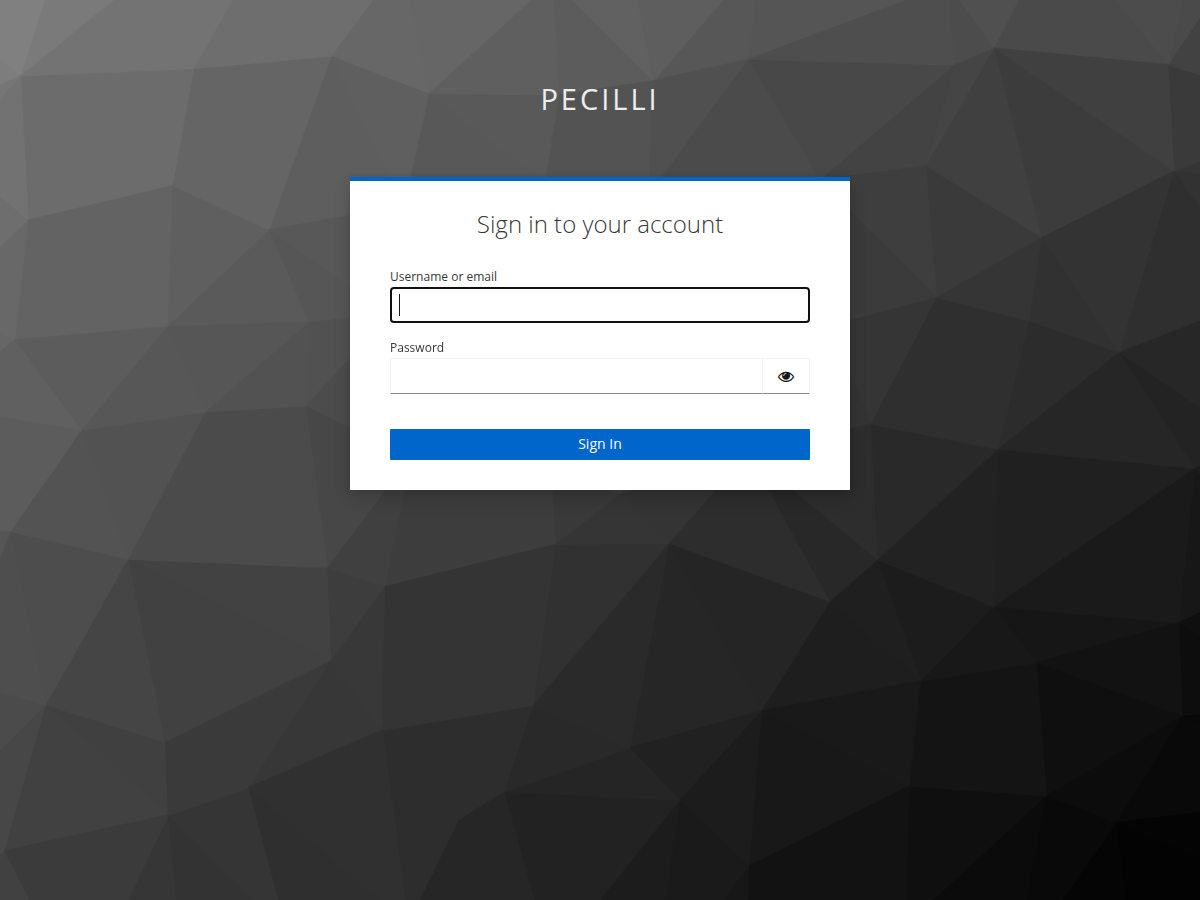
\includegraphics[width=0.72\textwidth]{Images/screenshots/ui-keycloak-login.png}
\caption{Schermata di accesso Keycloak al realm \texttt{pecilli}, intermedia
fra il browser e la dashboard nativa.}
\label{fig:ui-keycloak}
\end{figure}

\section{Sicurezza e osservabilità}

Il prototipo prevede le seguenti misure per l'interfaccia e l'accesso alle
fonti esterne:

\begin{itemize}
    \item accesso all'interfaccia tramite Keycloak (OIDC) con ruoli applicativi;
    \item credenziali e URL remoti forniti tramite variabili d'ambiente;
    \item validazione degli URL di dettaglio GDACS, limitati a host ufficiali;
    \item schemi Pydantic per rifiutare forme non valide (non la correttezza
    semantica di luogo o periodo);
    \item nessuna azione distruttiva esposta dai tool MCP;
    \item contenuti esterni trattati come dati, non come istruzioni;
    \item filtraggio dei dati sensibili nei log applicativi;
    \item correlazione fra risposta e log tramite
    \texttt{request\_id}/\texttt{thread\_id} e header diagnostici.
\end{itemize}

Il prototipo è descritto nella configurazione di sviluppo: l'accesso OIDC
all'interfaccia e la separazione dei checkpoint per conversazione non
costituiscono una valutazione della sicurezza delle API in produzione.

I log strutturati includono \texttt{request\_id}, \texttt{thread\_id},
servizio, durata, codice di errore e possibilità di retry. Gli endpoint
\url{/health/live}, \url{/health/ready} e
\url{/health?deep=true} distinguono stato del processo, dipendenze
obbligatorie e controlli remoti.

L'overlay osserva inoltre HTTP e SSE, workflow, nodi, chiamate LLM, tool MCP e
repository del grafo. Prometheus conserva le metriche e Grafana le visualizza;
OpenTelemetry esporta i trace a Phoenix. I trace possono catturare prompt e
output secondo configurazione e limiti: la protezione dei log non implica
l'assenza di contenuti nella telemetria. Il Capitolo~\ref{cap:6} descrive
copertura, interpretazione e limiti di questo livello.

Il vincolo trasversale dell'architettura riguarda i dati quantitativi: l'LLM può
selezionare un percorso o proporre una vista, ma non costituisce mai la sorgente
dei valori mostrati. Acquisizione, filtri, calcoli e validazione restano passaggi
eseguiti dal codice sui record recuperati.
